\documentclass[handout]{beamer}

\input{../ts-glærur}

\title{FOR3R - Röðunarreiknirit I}

\begin{document}
\begin{frame}
\titlepage
\end{frame}

\section{Röðunarvandamálið}

\begin{frame}{Röðunarvandamálið}
Sum vandamál skjóta oftar upp kollinum en önnur, þar á meðal er vandamál kallað \emph{röðunarvandamálið}:

\begin{framed}
\texttt{RÖÐUN TALNA}

\textbf{Inntak:} Runa talna, $\{a_1, a_2, \ldots, a_n\}$

\textbf{Úttak:} Endurröðun talnanna, $\{a_1', a_2', \ldots, a_n'\}$ svo að $a_1' \leq a_2' \leq \ldots \leq a_n'$
\end{framed}

Venjulega er runan táknuð sem listi eða fylki talna.
\end{frame}

\begin{frame}[fragile]
\begin{itemize}
 \item Við munum eyða nokkrum tíma í að skoða röðunarvandamálið.
 \item Ekki endilega vegna þess að það er svo áhugavert í sjálfu sér\ldots
 \pause
 \item en til að leysa það eru til mýmörg áhugaverð reiknirit.
 \pause
 \item Af hverju ekki bara að nota innbyggðu reikniritin?
 \begin{minted}{python}
 >>> sorted([2, 5, 4, 3, 1])
 [1, 2, 3, 4, 5]
 \end{minted}
 \pause
 \item \href{http://envisage-project.eu/proving-android-java-and-python-sorting-algorithm-is-broken-and-how-to-fix-it/}{Yfirleitt} er það það sem við viljum. En við getum lært af aðferðunum við að skrifa þær.
\end{itemize}
\end{frame}


\section{Selection Sort}

\begin{frame}{Selection Sort}
\begin{itemize}
 \item Einfalt röðunarreiknirit sem við höfum þegar kynnst er \emph{Selection Sort}. Því má lýsa á eftirfarandi hátt:
 \begin{enumerate}
  \item Listanum er skipt í tvo hluta: Röðuðum hluta (til ``vinstri'') og óröðuðum (``til hægri''). Í upphafi er raðaði hlutinn tómur og óraðaði hlutinn allur listinn.
  \item Ítrað er í gegnum óraðaða hluta listans og minnsta stakið í þeim hluta er fundið.
  \item Skipt er á staðsetningu staksins sem fannst í liðnum á undan og því staki sem lengst er til vinstri í óraðaða listanum.
  \item Mörk undirlistanna eru færð eitt skref til hægri.
 \end{enumerate}
\end{itemize}
\end{frame}

\begin{frame}{Selection Sort: YouTube}
\url{http://www.youtube.com/watch?v=92BfuxHn2XE}
\end{frame}

\begin{frame}[fragile]{Selection Sort: Python-kóði}
\inputminted[linenos]{python}{Code/Python/selection_sort.py}
\end{frame}

\begin{frame}[fragile]{Selection Sort: Python-kóði + tímaflækjugreining}
\inputminted[linenos]{python}{Code/Python/selection_sort_complexity.py}
\end{frame}

\begin{frame}[fragile]{Selection Sort: Endurkvæmur Python-kóði}
Endurkvæmni og lykkja notuð saman
\inputminted[linenos]{python}{Code/Python/selection_sort_recursive.py}
(Ath: Ekki ``in-place'')
\end{frame}

\section{Insertion Sort}

\begin{frame}{Insertion Sort}
\begin{itemize}
 \item Insertion Sort er ``einfalt'' en töluvert notað reiknirit
 \item Skalast verr (verri tímaflækja) en sum önnur reiknirit, en er hagkvæm fyrir mjög lítil inntök
 \item Virkar vel á inntök sem þegar eru í nokkuð góðri röð
 \item ``Online''
 \begin{itemize}
  \item Mikilvægara í gamla daga?
 \end{itemize}
 \item Mannfólk notar oftast einhvers konar Insertion Sort til að raða hlutum
\end{itemize}
\end{frame}

\begin{frame}{Insertion Sort - Lýsing}
\begin{itemize}
 \item Fyrir hvert stak í inntakinu skal gera eftirfarandi (frá vinstri til hægri):
 \begin{itemize}
  \item Vista gildi staksins
  \item Bera gildi staksins saman við öll stök sem á undan koma í listanum (frá hægri til vinstri)
  \begin{itemize}
   \item Sé gildið minna en samanburðarstakið afritum við það í næsta sæti til hægri
   \item Sé gildið ekki minna en samanburðarstakið setjum við það í sæti samanburðarstaksins
  \end{itemize}
 \end{itemize}
\end{itemize}
\end{frame}

\begin{frame}[fragile]{Insertion Sort - Sauðakóði}
\begin{center}
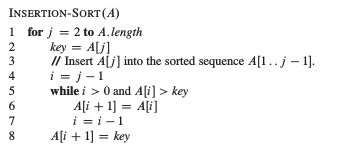
\includegraphics[width=0.7\textwidth]{Pics/InsertionSort}
\end{center}
Sjá betur: Introduction to Algorithms, bls. 18
\end{frame}

\begin{frame}{Insertion Sort: YouTube}
Útgáfa af Insertion Sort sem notar ``swaps'' inni í lykkjunni (af Wikipedia):
\begin{center}
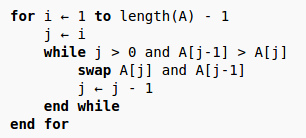
\includegraphics[width=0.7\textwidth]{Pics/InsertionSortSwaps}
\end{center}
\url{http://www.youtube.com/watch?v=8oJS1BMKE64}
\end{frame}

\begin{frame}{Tímaflækja Insertion Sort}
\begin{itemize}
 \item Tímaflækja Insertion Sort er mjög háð eðli inntaksins
 \begin{itemize}
  \item Hvað gerist ef inntakið er þegar raðað?
  \item Hvað gerist ef inntakið er í öfugri röð?
  \item Hvað gerist í ``meðaltilvikinu''?
 \end{itemize}
\end{itemize}

\end{frame}


\section{Önnur (fánýtari) röðunarreiknirit}
\begin{frame}{Fánýtari röðunarreiknirit}
\begin{itemize}
 \item \href{https://en.wikipedia.org/wiki/Bubble\_sort}{Bubble Sort}
 \item \href{https://en.wikipedia.org/wiki/Gnome\_sort}{Gnome Sort}
 \item Og það verður verra\ldots
 \begin{itemize}
  \item Bogosort
  \item Stooge sort
  \item Sleepsort
 \end{itemize}
\end{itemize}

\end{frame}

\end{document}
